\chapter{Compilation - Leiserson MIT}
\section{Interpreters vs Compilers}
Interpreted languages are more versatile, but much slower.
\begin{lstlisting}
for (int i = 0; i < n; i++) {
   for (int j = 0; j < n; j++) {
      for (int k = 0; k < n; k++) {
         C[i][j] += A[i][k] +B[k][j];
      }
   }
}
\end{lstlisting}
This code executed using Clang/LLVM 5.0 takes 1156s (19m 16s) to execute, about \textbf{2x} times faster than Java and \textbf{18x} times than python


\section{Cache}
\begin{paracol}{2}
   \colfill
   \begin{lstlisting}
      for (int i = 0; i < n; i++) {
            for (int k = 0; k < n; k++) {
         for (int j = 0; j < n; j++) {
               C[i][j] += A[i][k] +B[k][j];
            }
         }
      }
   \end{lstlisting}
   \colfill

   We can change the order of the loops without changing the result, but the performance can change.

   \switchcolumn

   \begin{figure}[htbp]
      \centering
      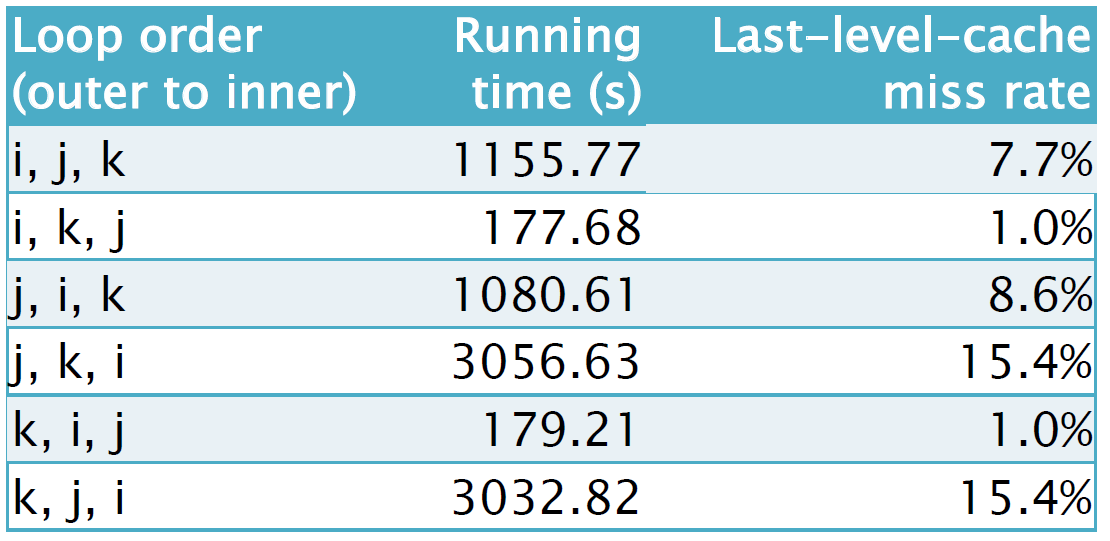
\includegraphics[width=0.9\columnwidth]{images/02/caches_looporder.png}
      \caption{Performance against loop order}
      \label{fig:caches_looporder}
   \end{figure}
   
\end{paracol}

As you can see, there is a huge difference in the running time of the loop depending on the loops ordering. This is due to \textbf{caching}, which consists in storing in a fast-access memory previously accessed memory lines.

\newpage
\begin{figure}[htbp]
   \centering
   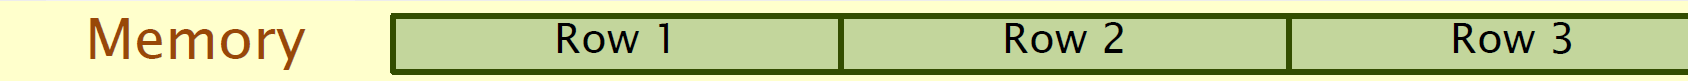
\includegraphics{images/02/rowmajor.png}
   \caption{Memory layout for matrix rows}
   \label{fig:rowmajor}
\end{figure}
Matrices are stored in memory in row-major order, so the first loop should iterate over the rows of the matrix, to exploit the cache.

\begin{figure}[htbp]
   \centering
   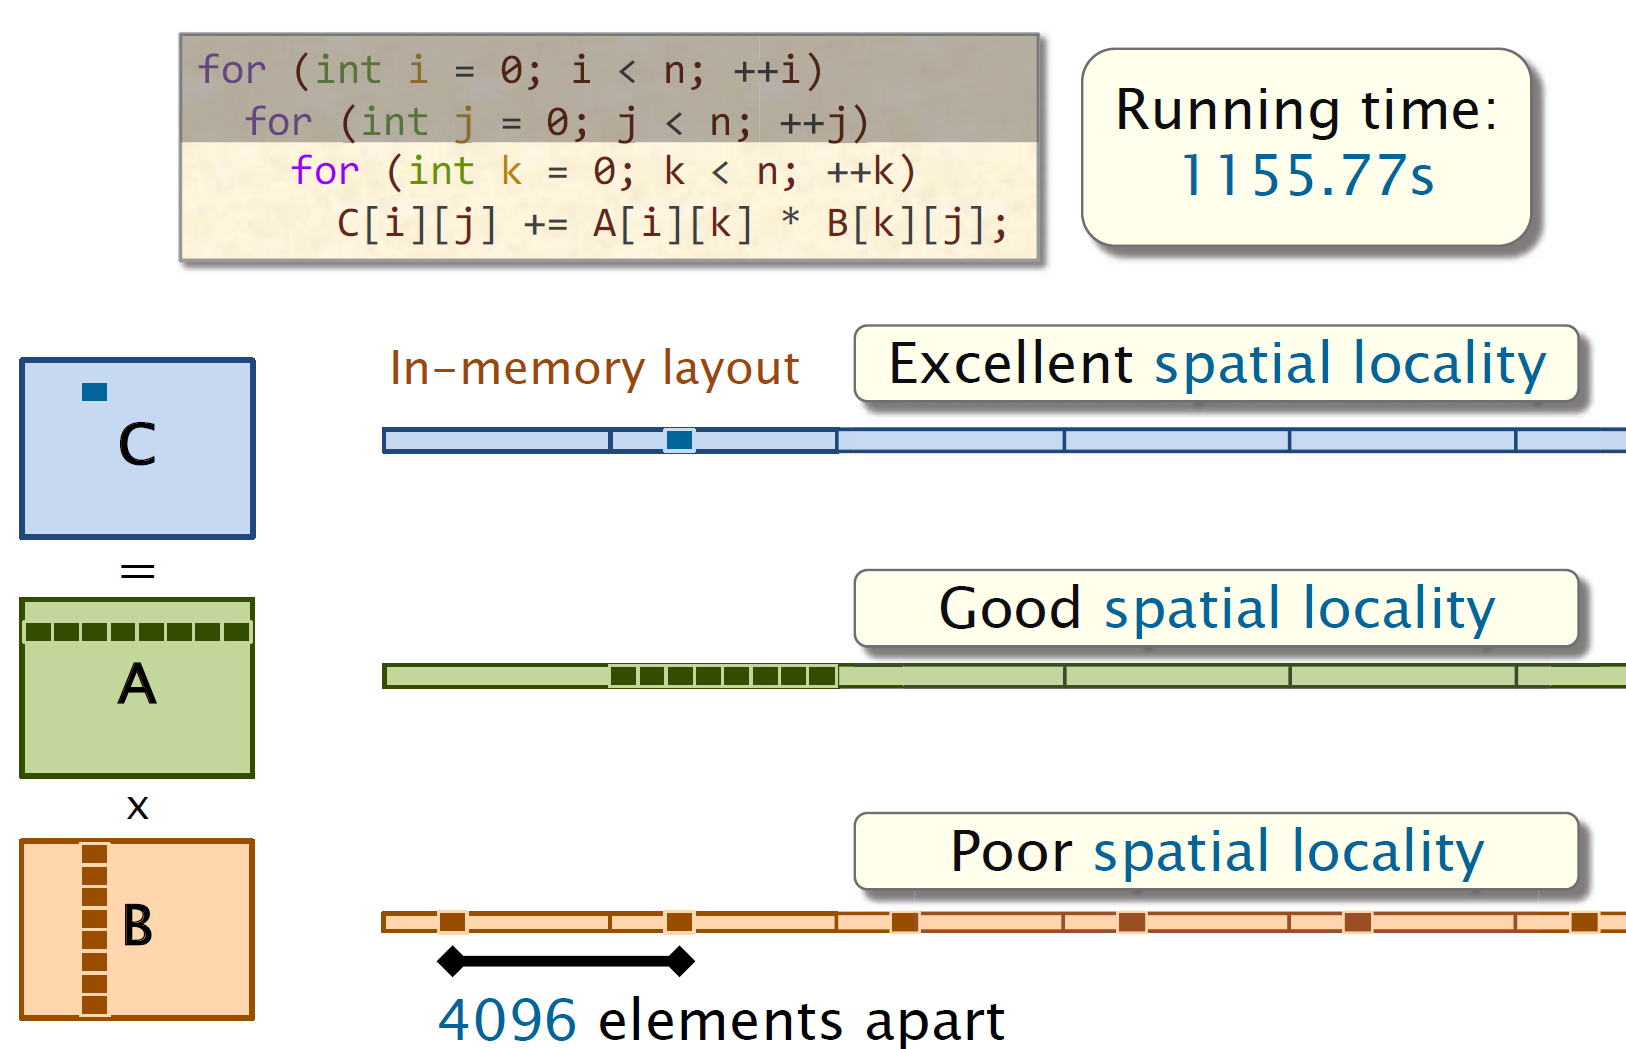
\includegraphics[width=0.49\columnwidth]{images/02/memory_layout1.png}
   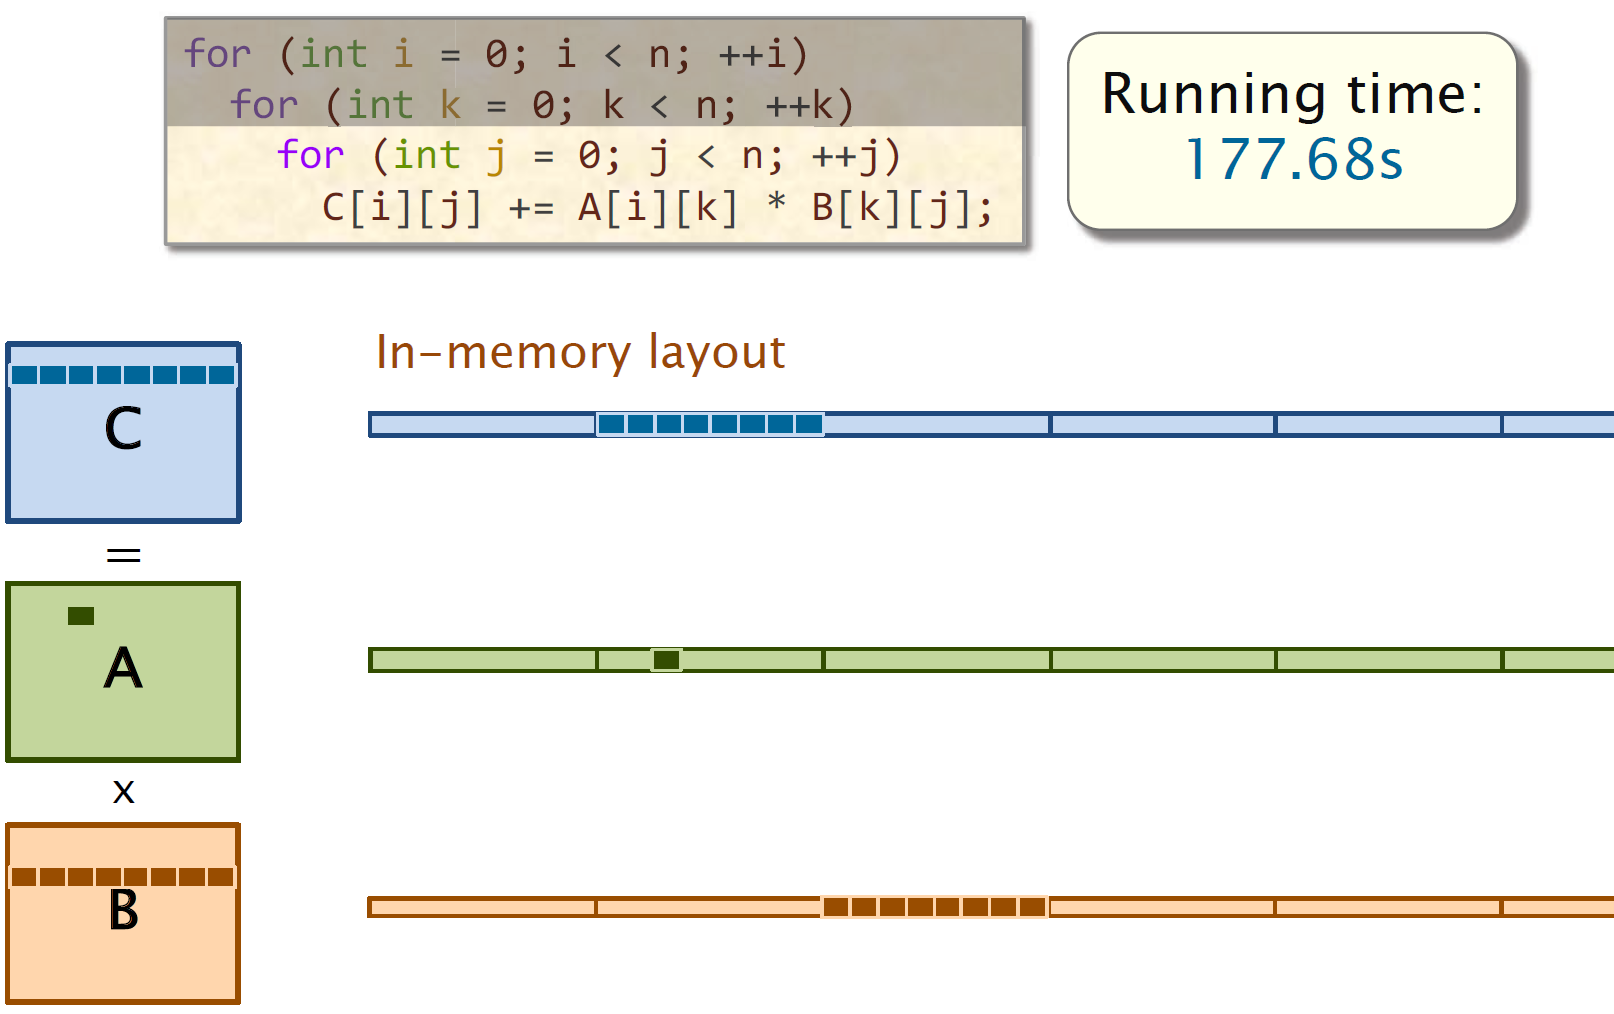
\includegraphics[width=0.49\columnwidth]{images/02/memory_layout2.png}\\
   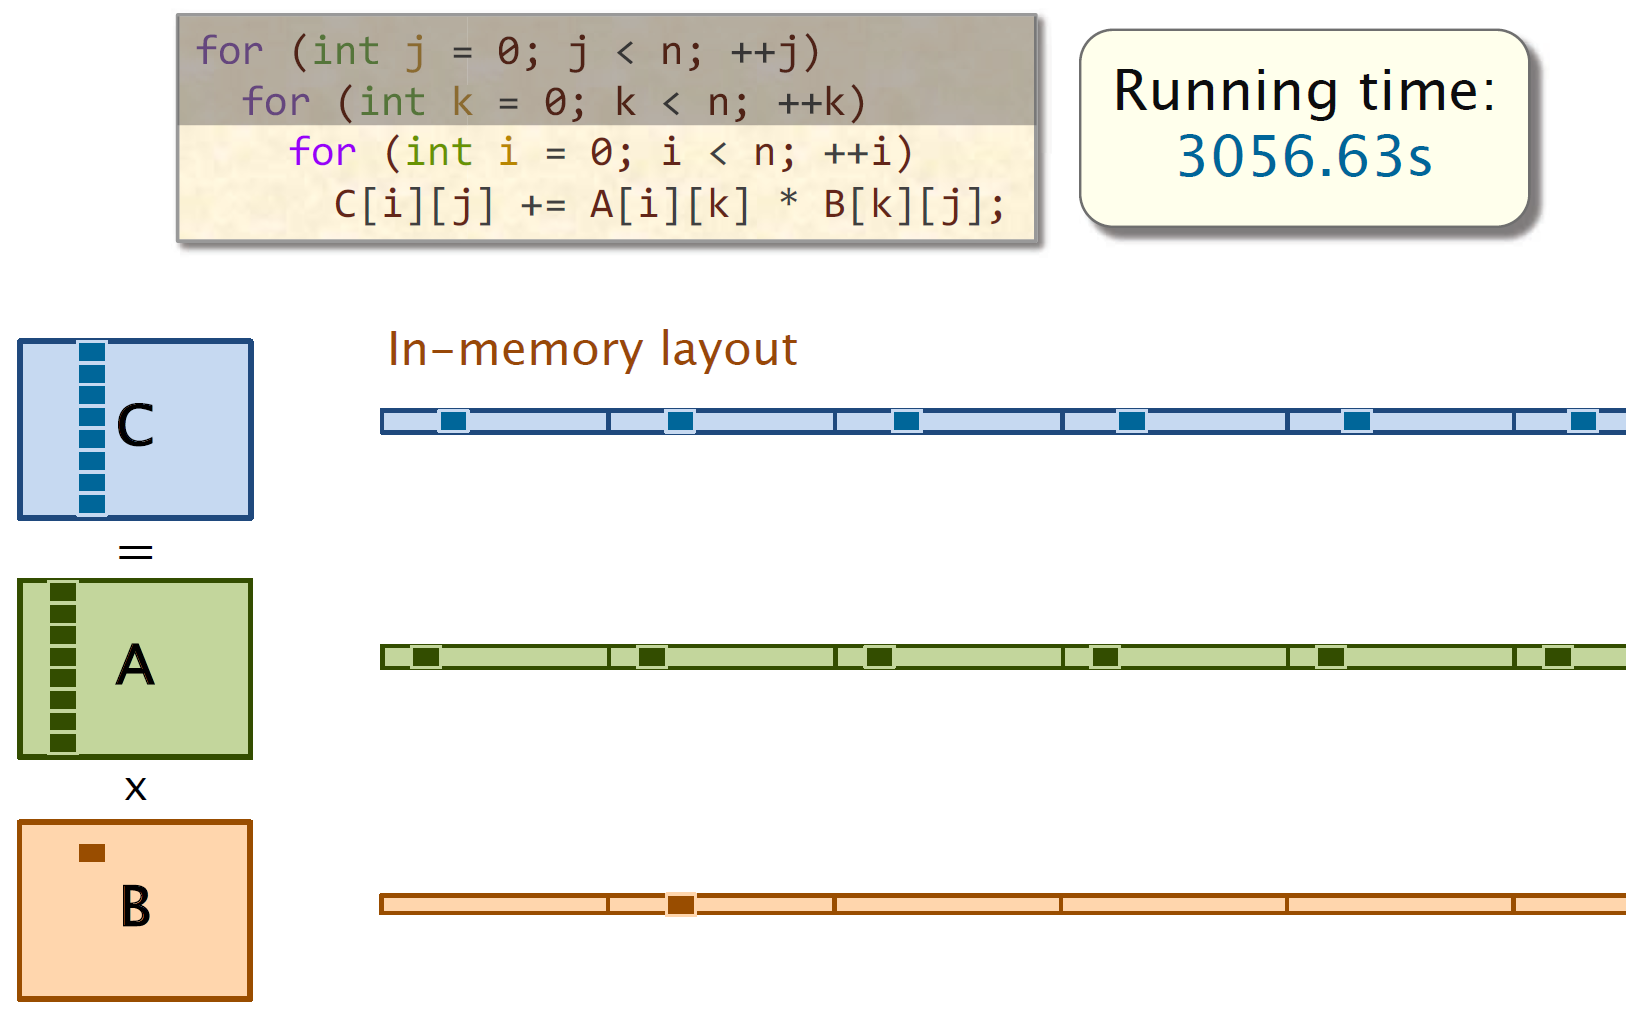
\includegraphics[width=0.49\columnwidth]{images/02/memory_layout3.png}
   \caption{Memory layout and spaciality implications}
   \label{fig:spaciality}
\end{figure}

\section{Compiler Optimization}
\begin{paracol}{2}
   \colfill
   Clang offers a lot of optimization flags, like \texttt{-O3} which enables all the optimizations. The compiler can also unroll loops, which means that it can execute multiple iterations of the loop in parallel. This can be done only if the number of iterations is known at compile time.
   There are also \texttt{-0s} which optimizes for size, and \texttt{-0g} which generates debug information. There's plenty of them, for various uses.
   \colfill
   
   \switchcolumn
   \begin{figure}[htbp]
      \centering
      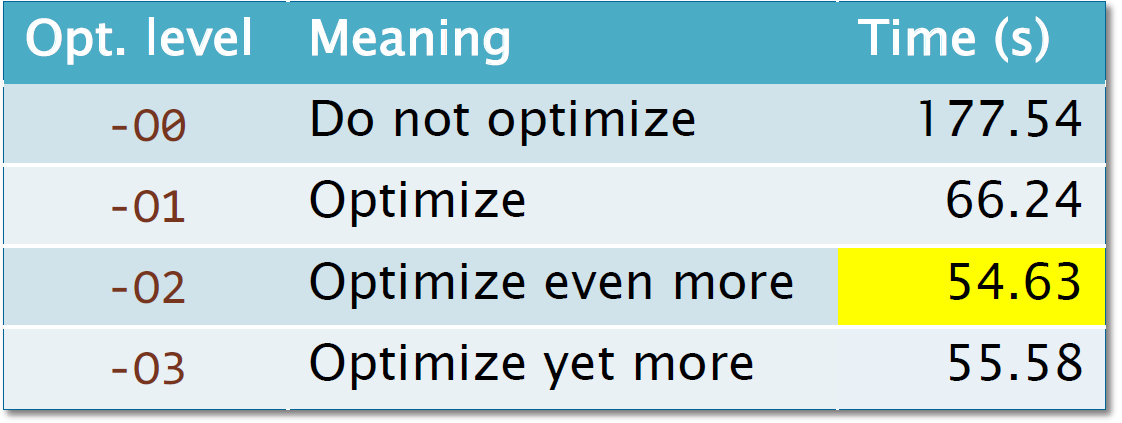
\includegraphics{images/02/optimization.png}
      \caption{Optimization flags and relative performance}
      \label{fig:optimization}
   \end{figure}
\end{paracol}

\section{Parallelizing}
Even after all these tweaks, we are still using only one of the 9 cores of the CPU.
So\dots
\begin{lstlisting}
   cilk_for (int i = 0; i < n; i++) {
      for (int k = 0; k < n; k++) {
         cilk_for (int j = 0; j < n; j++) {
            C[i][j] += A[i][k] +B[k][j];
         }
      }
   }
\end{lstlisting}
We don't have to know what's behind the \texttt{cilk\_for} keyword, but it will parallelize the \texttt{for} loop execution.
\framedt{
   But which \texttt{for} loops should we parallelize?
}{
   Parallelizing all three would cause multiple threads to access the same memory, which would be messy.

   A \ul{\textbf{rule of thumb} is to parallelize the \textbf{outermost} loop}, which is the one that iterates over the rows of the matrix.
   
   This is demonstrated by the following slide. 
}

\begin{figure}[htbp]
   \centering
   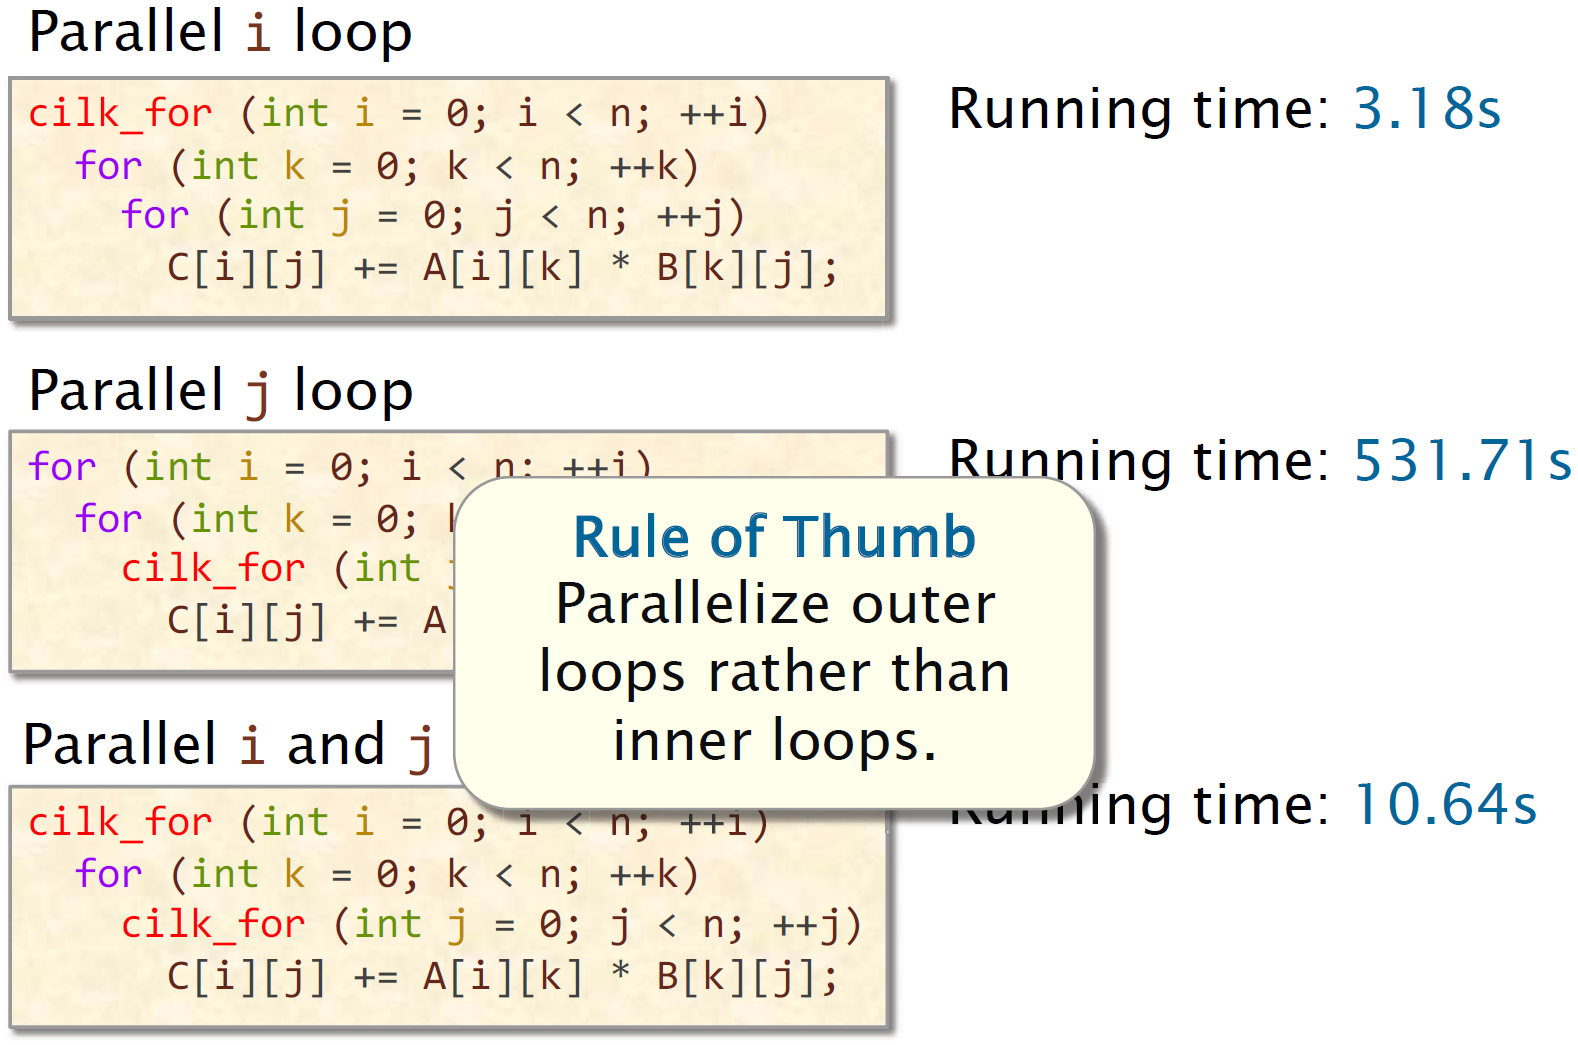
\includegraphics{images/02/loops_rule_of_thumb.png}
   \caption{Parallelizing only the outermost loop leads to optimal performance}
   \label{fig:loops_rule_of_thumb}
\end{figure}